%%%%%%%%%%%%%%%%%%%%%%%%%%%%%%%%%%%%%%%%%
% Structured General Purpose Assignment
% LaTeX Template
%
% This template has been downloaded from:
% http://www.latextemplates.com
%
% Original author:
% Ted Pavlic (http://www.tedpavlic.com)
%
% Note:
% The \lipsum[#] commands throughout this template generate dummy text
% to fill the template out. These commands should all be removed when
% writing assignment content.
%
%%%%%%%%%%%%%%%%%%%%%%%%%%%%%%%%%%%%%%%%%

%----------------------------------------------------------------------------------------
%	PACKAGES AND OTHER DOCUMENT CONFIGURATIONS
%----------------------------------------------------------------------------------------

\documentclass{article}

\usepackage{fancyhdr} % Required for custom headers
\usepackage{lastpage} % Required to determine the last page for the footer
\usepackage{extramarks} % Required for headers and footers
\usepackage{graphicx} % Required to insert images
\usepackage{amsmath,amsfonts,amsthm}
\usepackage{cancel}
\usepackage{multicol}
\usepackage{color}
\usepackage{soul}
\usepackage{multirow}

\newcommand{\hilight}[1]{\colorbox{yellow}{#1}}

% Margins
\topmargin=-0.45in
\evensidemargin=0in
\oddsidemargin=0in
\textwidth=6.5in
\textheight=9.0in
\headsep=0.25in

\setlength\parindent{0pt}
\linespread{1.5}
\allowdisplaybreaks

\newcommand{\bx}{\mathbf{x}}
\newcommand{\bff}{\mathbf{f}}
\newcommand{\bG}{\mathbf{G}}
\newcommand{\bg}{\mathbf{g}}
\newcommand{\bu}{\mathbf{u}}
\newcommand{\by}{\mathbf{y}}
\newcommand{\bxh}{\hat{\mathbf{x}}}
\newcommand{\byh}{\hat{\mathbf{y}}}
\newcommand{\bffh}{\hat{\mathbf{f}}}
\newcommand{\bGh}{\hat{\mathbf{G}}}
\newcommand{\bgh}{\hat{\mathbf{g}}}
\newcommand{\bxb}{\bar{\mathbf{x}}}
\newcommand{\diag}{\mathrm{diag}}
\newcommand{\xh}{\hat{x}}
\newcommand{\bz}{\mathbf{0}}
\newcommand{\bk}{\mathbf{k}}
\newcommand{\Deltah}{\hat{\Delta}}
\newcommand{\be}{\mathbf{e}}

%----------------------------------------------------------------------------------------

\begin{document}
\large
2016-02-16

\section*{Comparison on communciation cost}
\begin{figure}[h!]
    \centering
    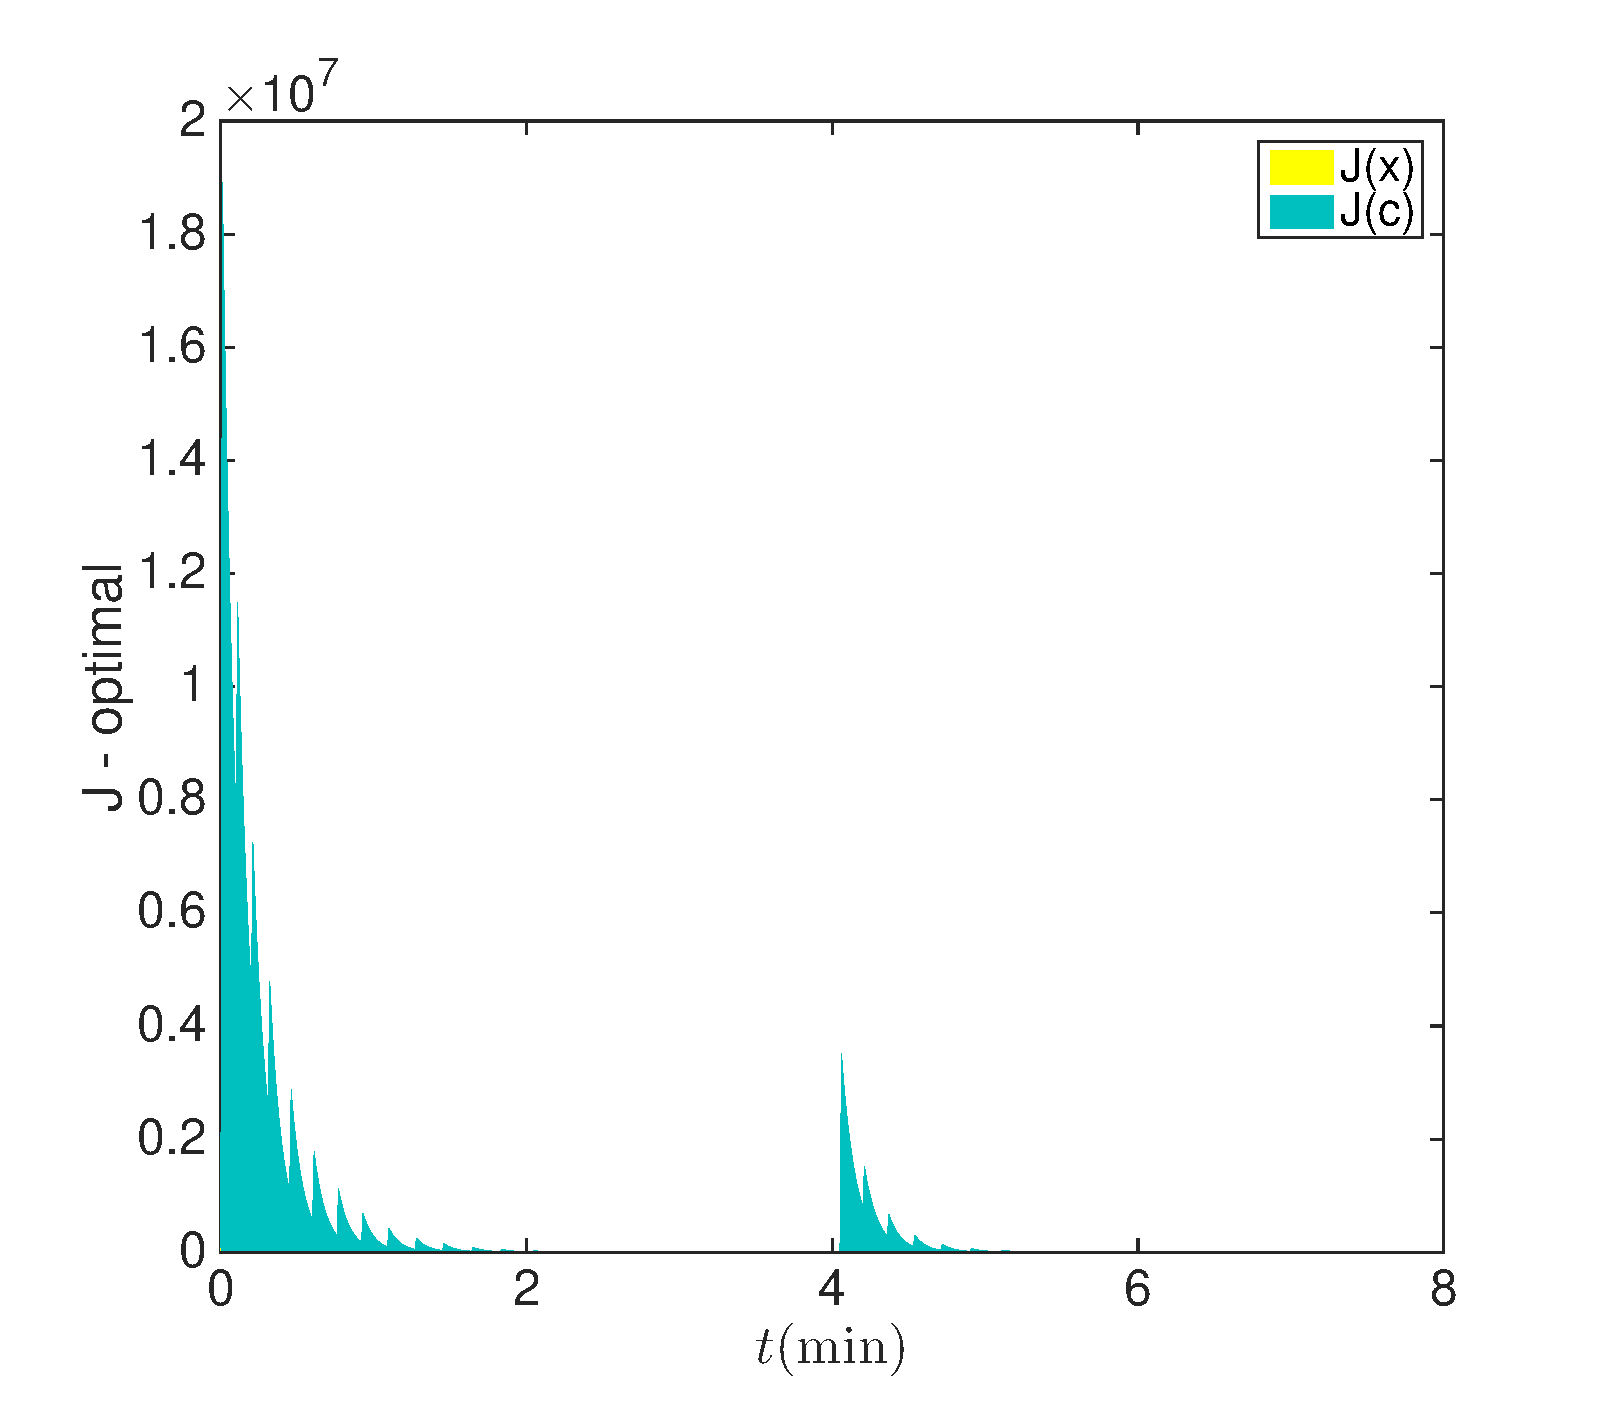
\includegraphics[width=0.45\linewidth]{Cost_optimal}
    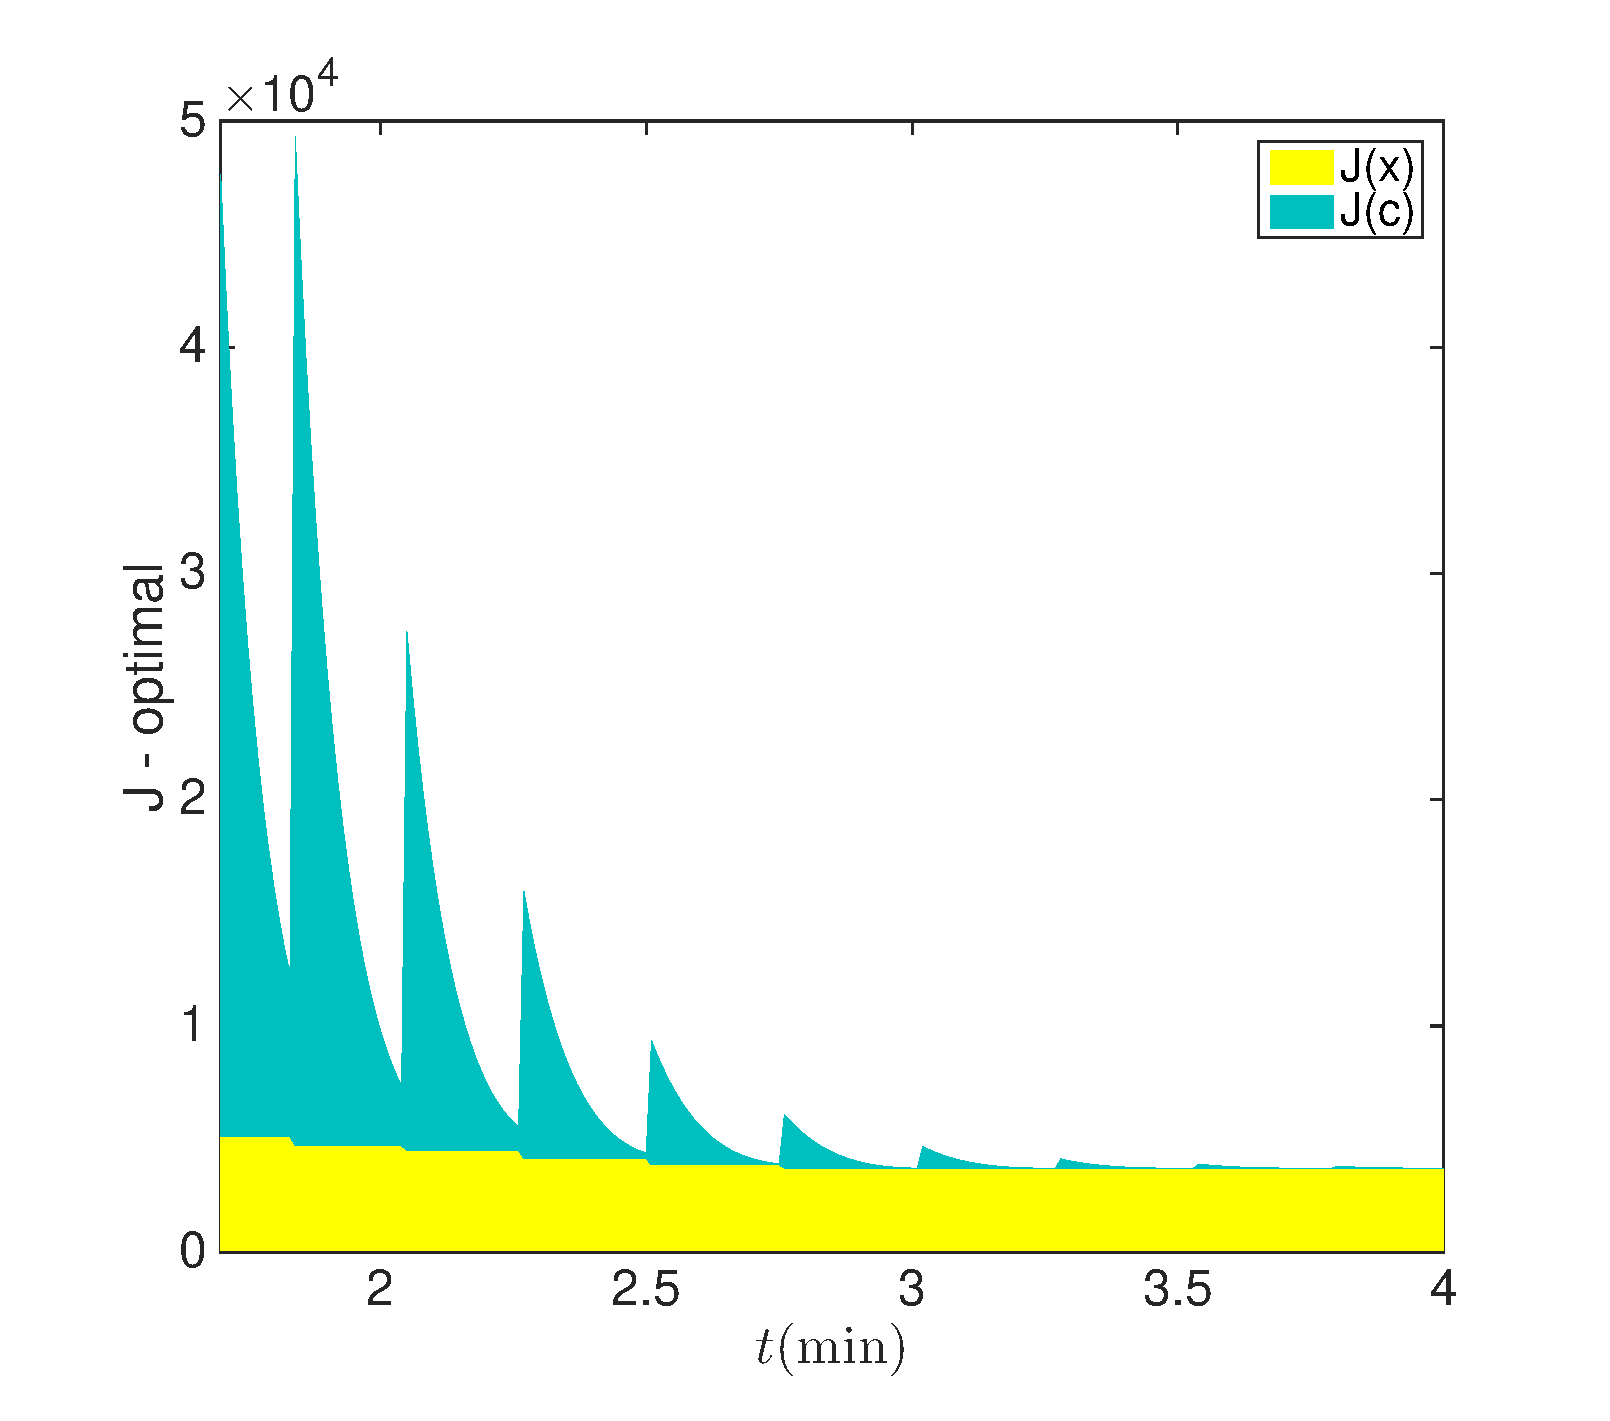
\includegraphics[width=0.45\linewidth]{Cost_optimal_zoom}
    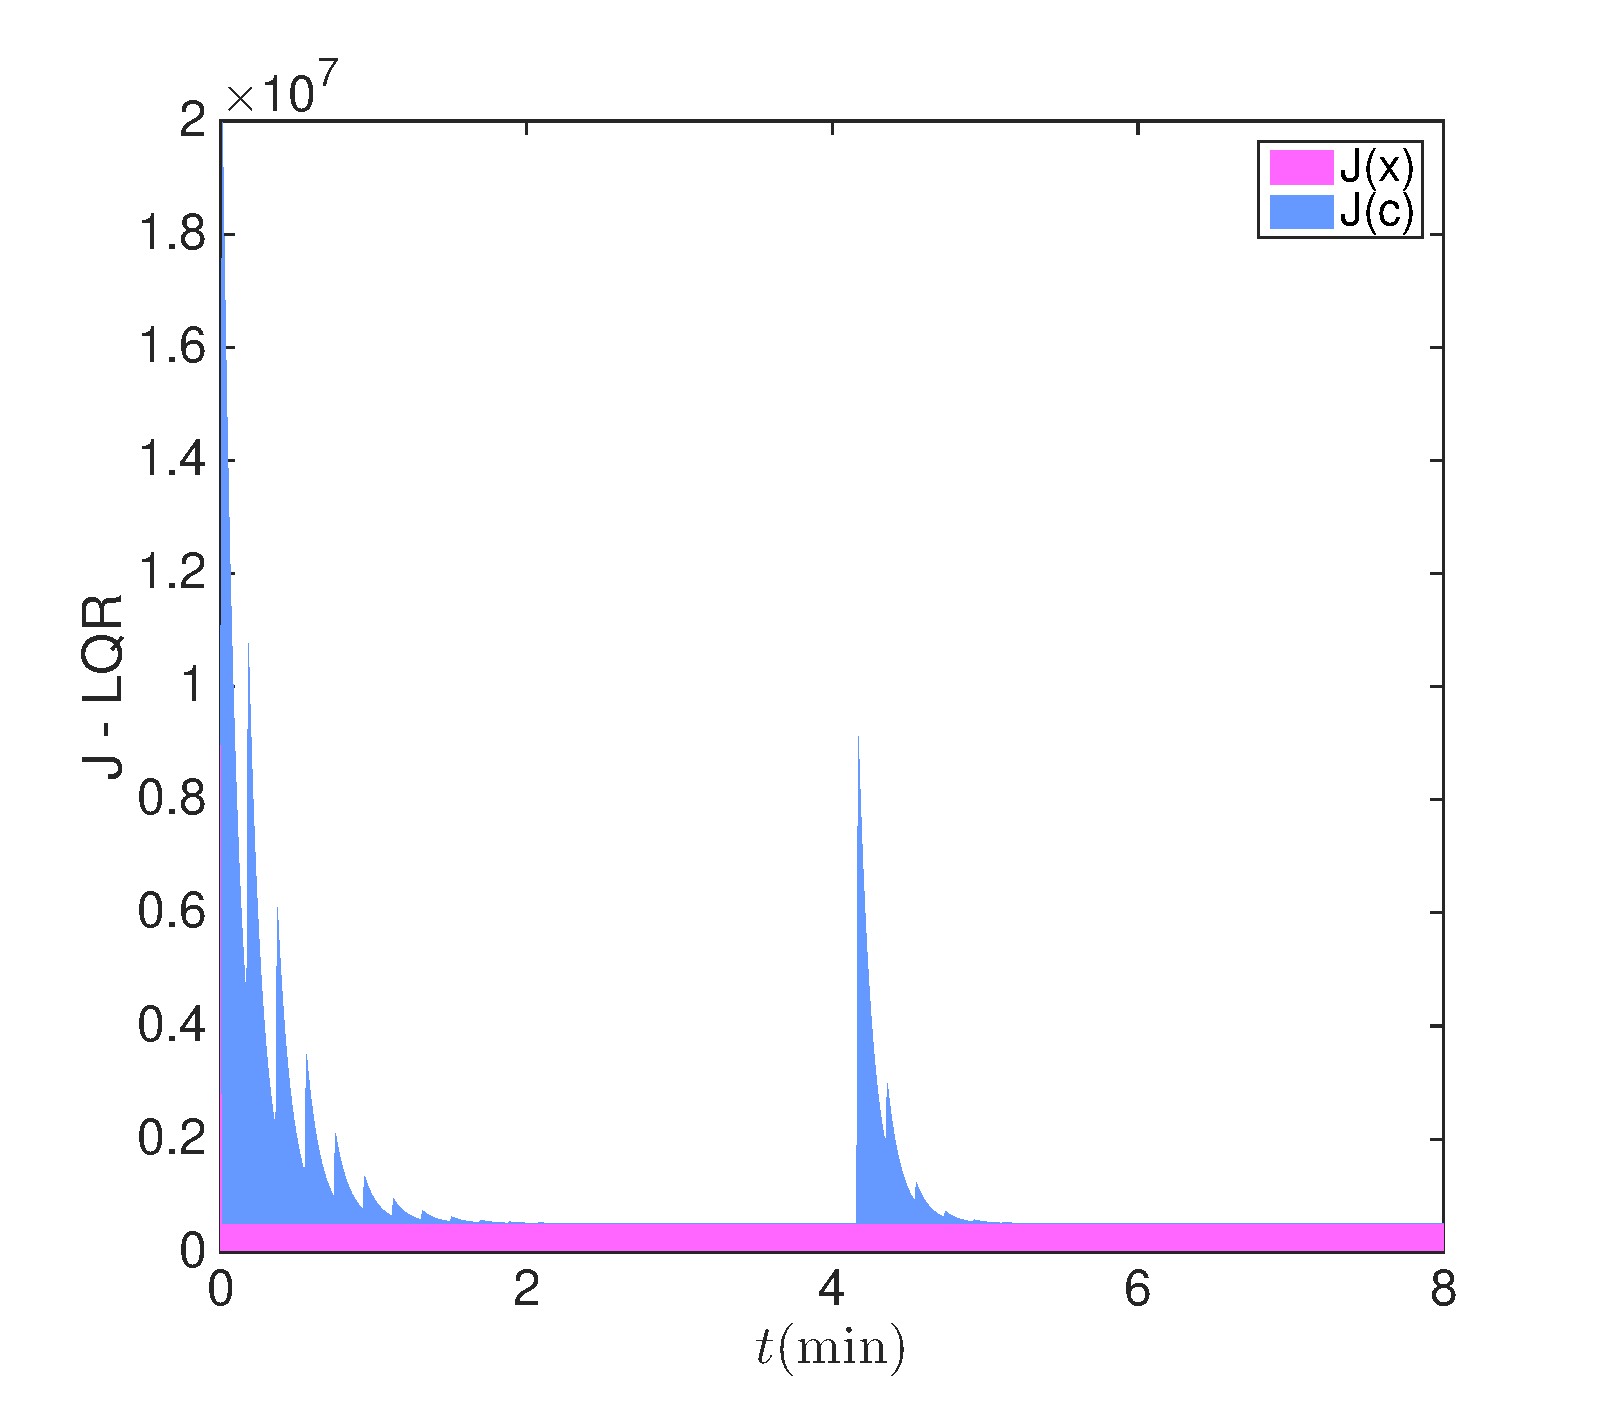
\includegraphics[width=0.45\linewidth]{Cost_lqr}
    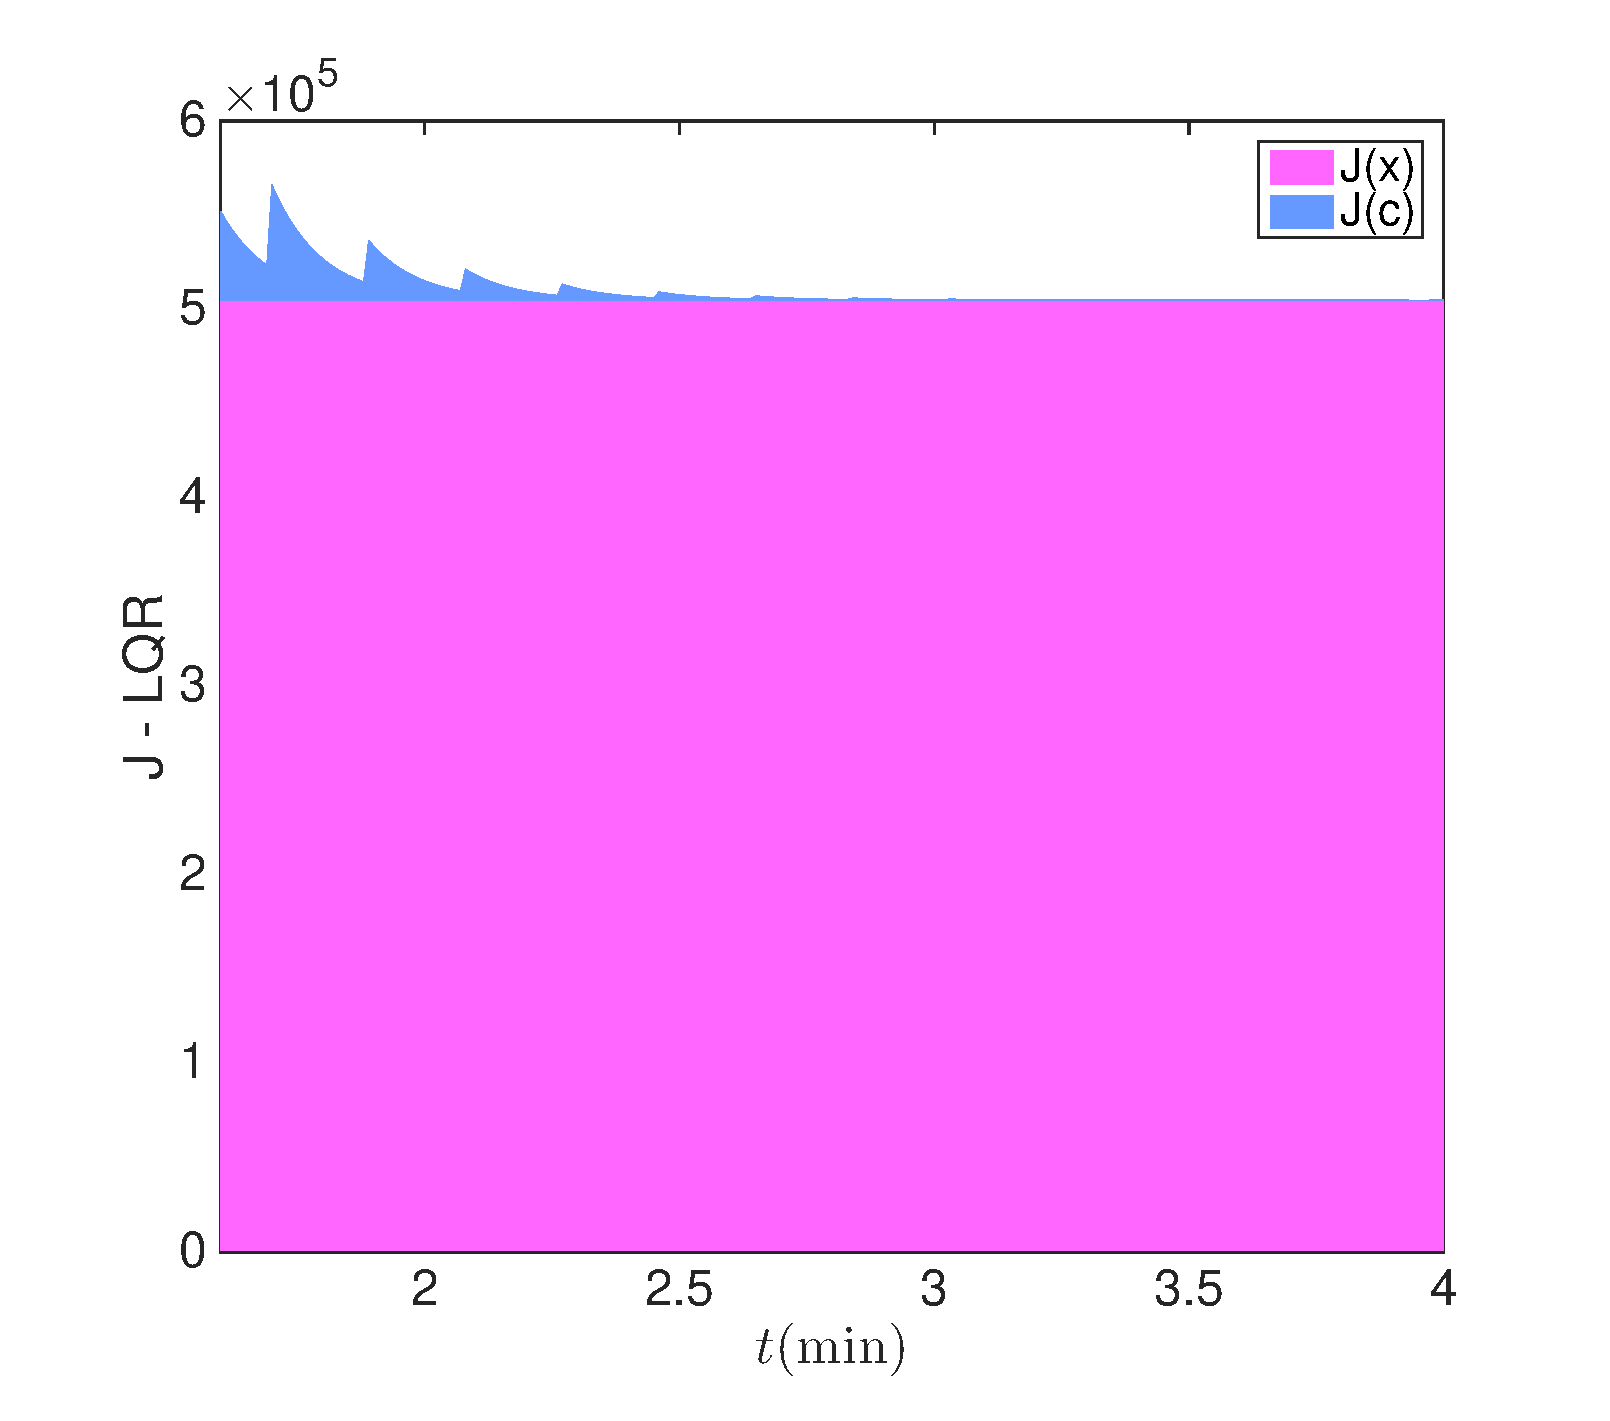
\includegraphics[width=0.45\linewidth]{Cost_lqr_zoom}
    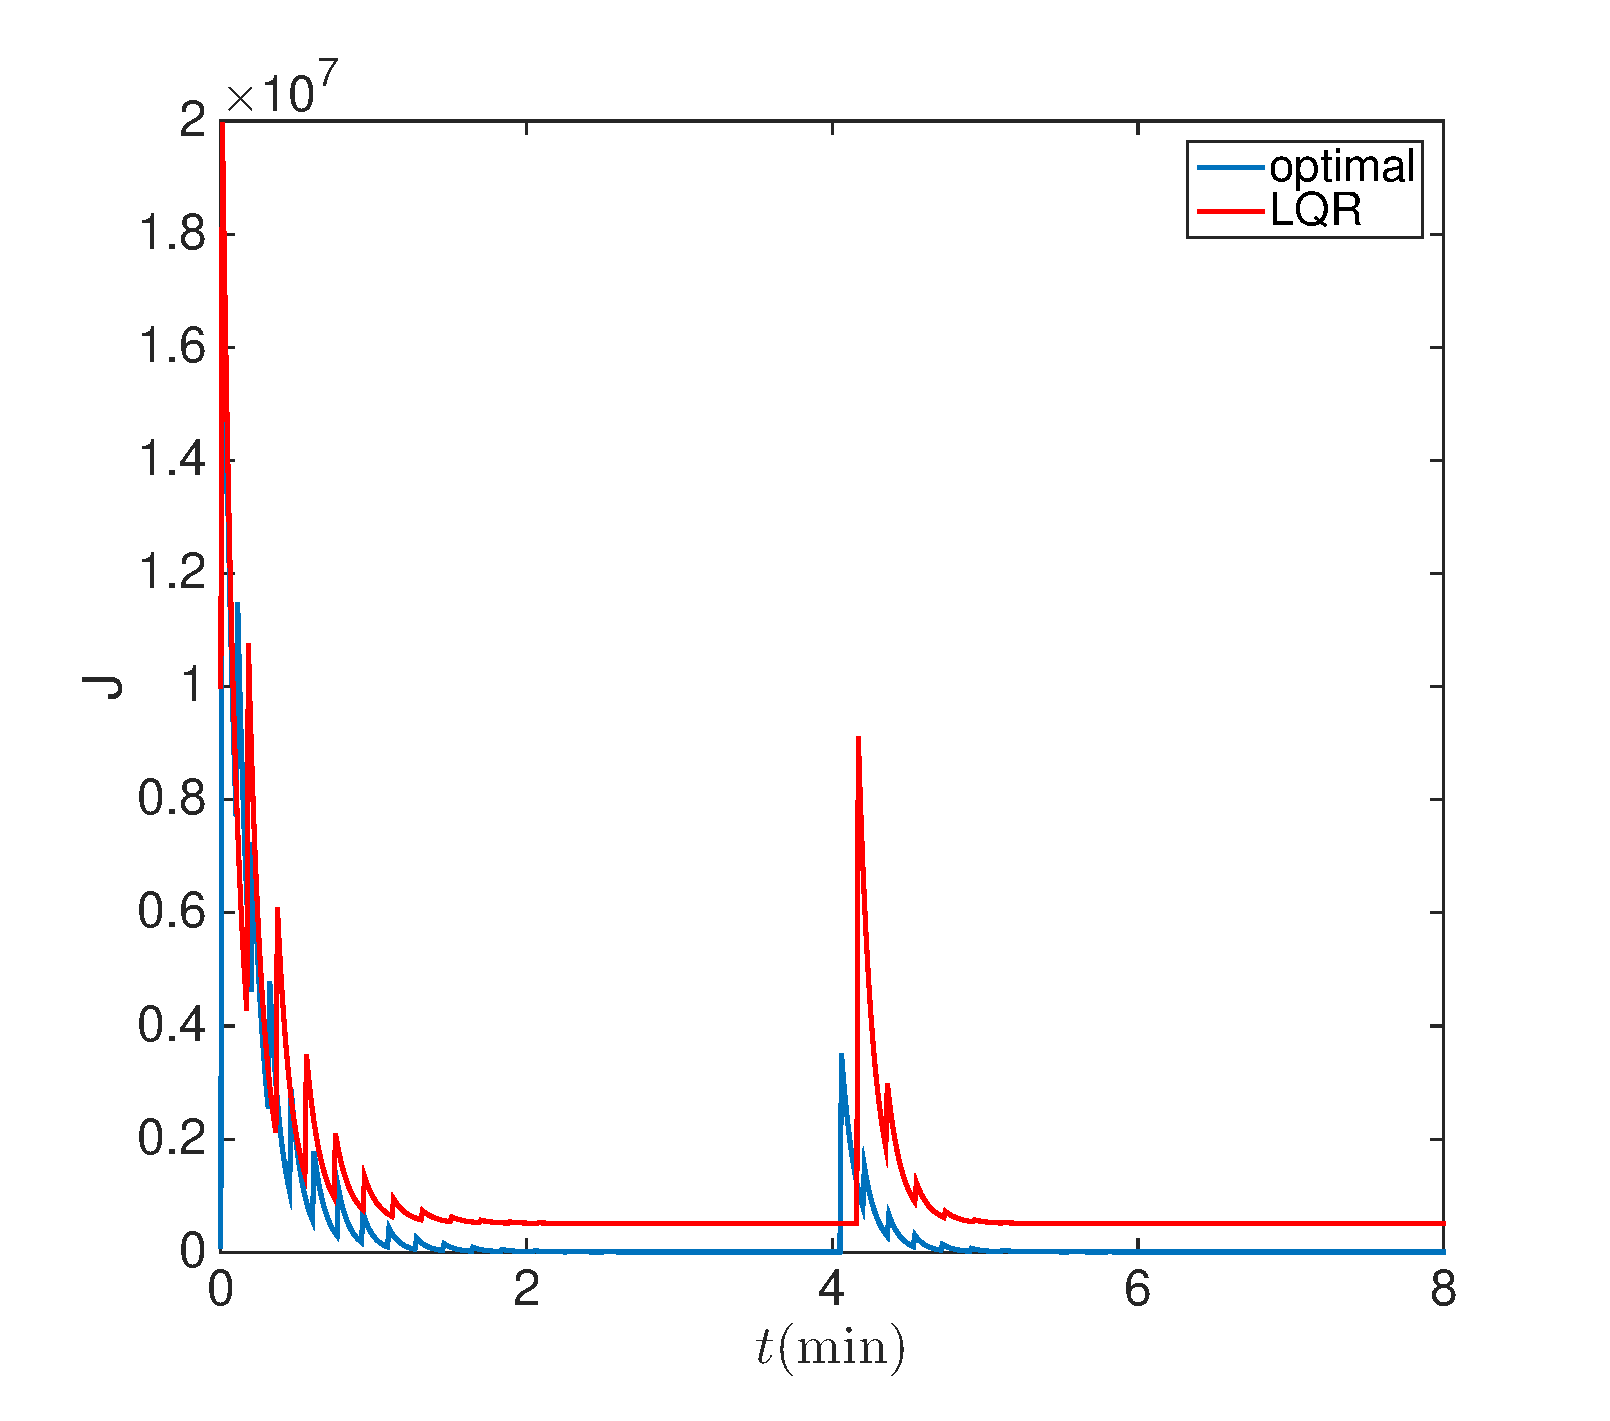
\includegraphics[width=0.45\linewidth]{Cost_compare}
\end{figure}
 

\begin{table}
\centering
\caption{Comparison on operating costs}
\begin{tabular}{lll}
\hline
Cost   & Optimal           & LQR               \\ \hline
$J(x)$ & $3.90\times 10^6$ & $4.66\times 10^6$ \\ \hline
$J(c)$ & $3.82\times 10^4$ & $4.14\times 10^6$ \\ \hline
Total  & $3.94\times 10^6$ & $8.80\times 10^6$ \\ \hline
\end{tabular}
\end{table}

\begin{table}
\centering
\caption{Comparison on operating cost break down}
\begin{tabular}{lll}
\hline
Percentage  & Optimal $(\%)$    & LQR $(\%)$    \\ \hline
$J(x)$      & 99.03             & 52.97         \\ \hline
$J(c)$      & 0.97              & 47.03         \\ \hline
\end{tabular}
\end{table}

Reduced over 50$\%$ of operating cost from the LQR: $\displaystyle{\frac{J_{\text{Opt}}}{J_{\text{LQR}}}} \times 100 \%= 44.74 \%$.



\end{document}

